%!TEX root = TQFTbook.tex
%%%%%%%%%%%%%%
\chapter{Lattice construction of extended 2d TQFT}\label{c:2d-lattice}

In this chapter, we give an alternative approach to constructing 2d TQFT, based
on triangulating a manifold (or, more generally, choosing a PLCW decomposition,
as described in the previous chapter). In this approach, an invariant of a
closed 2-manifold is defined by a suitable sum over all ways of ``coloring''
cells of a given PLCW decomposition (we will explain it in more detail below).
In physics, such a sum is usually referred to as ``state sum''; it should be
considered a discretized analog of the path integral.

In the special case of DW theory, this approach is known as ``lattice gauge
theory'' and has been extensively studied by physicists. Generalization of
this to an arbitrary separable symmetric Frobenius algebra was suggested in
\cite{fhk}. See also \cite{oeckl}. Generalization to arbitrary symmetric
monoidal 2-categories is discussed in \cite{davidovich}.

Throughout this chapter, we fix a separable symmetric Frobenius algebra
$A$. As before, we assume that the ground field $\kk$ has characteristic 0.
We denote by $\eps \colon A\to \kk$ the counit. We also denote by
$(a,b)=\eps(ab)$ the corresponding bilinear pairing.
\section{Definition of TQFT via state sum}\label{s:state-sum}
As before, let $x_i$, $x^i$ be dual bases in $A$ with respect to the
Frobenius pairing. We denote by $g_{ij}$ the matrix of the pairing in
the basis $x_i$: $g_{ij}=(x_i,x_j)$ and by $g^{ij}$ the inverse matrix:
$\sum_{j} g_{ij}g^{jk}=\de_{ik}$. We will use $g_{ij}$, $g^{ij}$ for
raising and lowering indices of various tensors.

For any $k \ge 0$, define the map $A^k\to \kk$ by
\begin{equation}\label{e:k-pairing}
\< a_1, \dots, a_k\> = \eps (a_1\cdot \dots \cdot a_k).
\end{equation}

\begin{lemma}\label{l:k-pairing}
  \par\noindent
  \begin{enumerate}
    \item The map \eqref{e:k-pairing} is invariant under cyclic permutation of
      $a_i$:
      $$
      \< a_1, \dots, a_k\> = \<a_k, a_1, \dots, a_{k-1}\>.
      $$
    \item The map \eqref{e:k-pairing} is multilinear over $\kk$. Moreover, it is
      linear over $A$: for any $i=1,\dots, k$, $x\in A$, we have
      $$
        \< a_1, \dots, a_ix, a_{i+1},\dots, a_k\> =
        \< a_1, \dots, a_i, xa_{i+1},\dots, a_k\>
      $$
      \textup{(}for $i=k$, we take $a_{i+1}=a_1$\textup{)}.
    \item
      \begin{equation}\label{e:k-pairing-2}
        \sum_i \< a_1, \dots, a_k, x_i\> \< x^i, b_1, \dots, b_m\>
         =\< a_1, \dots, a_k, b_1, \dots, b_m\>
      \end{equation}
  \end{enumerate}
\end{lemma}
The proof of this lemma is straightforward and is left as an exercise to
the reader.

Let $M$ be a closed oriented 2-dimensional manifold. Let us choose a PLCW
decomposition $K$ of $M$ (see \seref{s:PLCW}), with the set of 2-cells $K_2$,
the set of 1-cells (edges) $K_1$, and the set of vertices $K_0$. We will denote
by $E$ the set of \emph{oriented} edges, i.e., pairs consisting of an edge $r\in
K_1$ and an orientation of $r$. Thus, every (unoriented) edge $r\in K_1$ gives
rise to two oriented edges $r', r''\in E$.

The invariant will be constructed by combining algebraic data defined by
2-cells, edges, and vertices of $M$, as defined below. The key ingredient of
this construction is the tensor product of copies of $A$, one copy for
each oriented edge $r$
\begin{equation}\label{e:AE}
  A^E = \bigotimes_{r\in E}A_r
\end{equation}
where we denote by $A_r$ a copy of $A$ corresponding
to $r$.

\subsubsection*{\textbf{Algebraic data determined by edges}}
Define, for each unoriented edge $r\in K_1$, an element
$$
 e_r = \sum x_i\otimes x^i
     =\sum g^{ij} x_i \otimes x_j\in A_{r'}\otimes A_{r''}
$$
where $r', r''$ are two possible orientations of $r$. Since $g^{ij}=g^{ji}$
(which follows from the symmetry of the form $(\, , \,)$), $e_r$ does not
depend on which of two possible orientations was denoted by $r'$ and which
by $r''$. Taking the product over all (unoriented) edges $r\in K_1(M)$, we
get an element
\begin{equation}\label{e:eM}
  e_M = \bigotimes_{r\in K_1} e_r\in A^E.
\end{equation}

\subsubsection*{\textbf{Algebraic data determined by vertices}}
Since $A$ is a separable Frobenius algebra, we have an invertible Euler element
$w=\sum x_ix^i\in z(A)$ (see \thref{t:separable-frobenius}). Choose now, for
every vertex $v\in K_0$ of the PLCW decomposition, an oriented edge $r(v)$
incident to $v$ ($v$ can be either the head or the tail of $r(v)$). Let the
operator
\begin{equation}\label{e:wv}
  w^{-1}_v\colon A^E\to A^E
\end{equation}
be the operator of left multiplication by $w^{-1}$ in the component $A_{r(v)}$.
Taking the product over all vertices, we get an operator
$$
\prod_v(w^{-1}_v)\colon A^E\to A^E.
$$
Note that this operator depends on the choice we made, namely the choice
of oriented edge for each vertex.

\subsubsection*{\textbf{Algebraic data determined by 2-cells}}

Every 2-cell $F\in K_2$ inherits a natural orientation from $M$. Thus, we
can define its boundary $\del F$. This is a collection of oriented edges,
which has a natural counterclockwise cyclic order.

We will actually be more interested in the boundary with reversed
orientation, writing $\ov{\del F}=\{r_1, \dots, r_k\}\subset E$; if we draw
$F$ as a polygon in $\R^2$ with the standard orientation, then the edges $r_i$
are oriented clockwise and taken in the natural clockwise order:

\begin{center}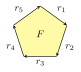
\includegraphics{figures/c12-fig01.svg}\end{center}

Define the map
\begin{align*}
\<\, \>_F\colon A^{\otimes \ov{\del F}}&\to \kk\\
                a_1\otimes \dots\otimes a_k&\mapsto \<a_1, \dots, a_k\>.
\end{align*}
\leref{l:k-pairing} implies that this map does not depend on which edge we
denote by $r_1$ and thus is well-defined.

\begin{remark}
  The reason for choosing $\ov{\del F}$ rather than $\del F$ is that we want
  to think of $F$ as a cobordism from $\ov{\del F}$ to the empty set.
\end{remark}

Since $M$ is a manifold, every unoriented edge appears twice as a boundary
edge of a 2-cell, and every oriented edge appears once as part of $\del F$.
Thus, by taking the tensor product of $\<\, \>_F$ over all 2-cells $F$, we
get a linear map
$$
  \bigotimes_F \< \, \>_F \colon A^E\to \kk.
$$

Let us now put it all together and define a number $Z_A(M,K)\in \kk$ by
\begin{equation}\label{e:fhk-state-sum}
  Z_A(M,K)= \Bigl(\bigotimes_F \< \, \>_F\Bigr)
          \Bigl(\prod_v(w^{-1}_v) \Bigr)e_M\in \kk
\end{equation}
where $e_M$ is defined by \eqref{e:eM} and $w_v$ is defined by \eqref{e:wv}.

%FIXME: picture with dual graphs.

\begin{theorem}\label{t:fhk1}
  Let $M$ be a closed oriented 2-manifold with PLCW decomposition $K$. Let
  $Z_A(M,K)$ be defined by \eqref{e:fhk-state-sum}.
  \begin{enumerate}
    \item So defined $Z_A(M,K)$ does not depend on the choice of an edge $r(v)$
      used to define $w^{-1}_v$.
    \item So defined $Z_A(M,K)$ does not depend on the choice of cell
      decomposition $K$.
  \end{enumerate}
\end{theorem}
\begin{proof}
  Part (1) follows from two observations:
  \begin{itemize}
    \item
      $$
      \sum w^{-1}x_i\otimes x^i=
      \sum x_i\otimes x^i w^{-1}=
      \sum x_i\otimes w^{-1}x^i
      $$
      (the first identity uses the centrality of $e$, the second uses the fact
      that  $w^{-1}$ is central). This shows that replacing a choice of edge
      $r(v)$ by the same edge but with opposite orientation does not change the
      vector $w^{-1}_ve_M$ and thus, does not change $Z_A(M,K)$.
    \item
      If $r_i$, $r_{i+1}$ are two edges of the boundary of some cell $F$ both
      adjacent to vertex $v$, as shown below, then replacing
      $r(v)=r_i$ by $r(v)= r_{i+1}$ does not change the composition
      $\Bigl(\bigotimes_F \< \, \>_F\Bigr)w^{-1}_v$ and thus, does not
      change $Z_A(M,K)$. Indeed, it follows from
      $\<\dots, a_{i}w^{-1}, a_{i+1}, \dots\> =
      \<\dots, a_{i}, w^{-1}a_{i+1}, \dots\>$.

      \begin{center}
      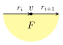
\includegraphics{figures/c12-fig02.svg}
      \end{center}

  \end{itemize}
  By using these two operations, we can replace any oriented edge adjacent
  to $v$ by any other edge. This proves part (1) of the theorem.

  To prove part (2), we need to verify that $Z_A(M,K)$ is invariant under
  elementary moves described in \firef{f:plcw-moves-2}.

  Invariance under subdivision of a 2-cell follows from \eqref{e:k-pairing-2}.

  Invariance under subdivision of a 1-cell follows from
  \begin{center}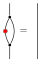
\includegraphics{figures/c12-fig03.svg}\end{center}
  where the red dot stands for the operator of multiplication by $w^{-1}$
  (which comes from the operator $w^{-1}_v$ for the newly added vertex). But
  this is immediate from the definition: indeed, comultiplication is given
  by $\De(a)=\sum a x_i \otimes x^i$, so the composition in the left-hand
  side is $a\mapsto \sum a x_i w^{-1}x^i=a$.
\end{proof}
\begin{remark}
  Note that without the $w^{-1}_v$ factor, this theorem would fail unless
  we assume $\sum x_ix^i=1$.
\end{remark}

Thus, we see that \eqref{e:fhk-state-sum} defines an invariant of closed
2-manifolds. In the next section, we will generalize it to manifolds with
boundary, thus defining an extended TQFT as a lattice theory.

\begin{example}\label{x:lattice-S2}
  Consider the PLCW decomposition of $S^2$ obtained by gluing together
  opposite edges of the bigon shown below.
  \begin{center}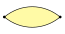
\includegraphics{figures/c12-eqfig01.svg}\end{center}
  This cell decomposition has one 2-cell, one 1-cell, and two vertices.
  The state sum \eqref{e:fhk-state-sum} in this case gives
  $$
    Z_A(S^2)=\sum \eps(w^{-2}x_ix^i)=\eps(w^{-1}).
  $$
\end{example}

\begin{example}\label{x:lattice-T2}
  Consider a PLCW decomposition of the torus $T^2$
  obtained by gluing together opposite sides of the rectangle. This
  decomposition has a single 2-cell, two edges, and one vertex.
  The state sum \eqref{e:fhk-state-sum} in this case gives
  $$
    Z_A(T^2)=\sum \eps(w^{-1}x_ix_jx^ix^j)=\sum (p(x_j),x^j)=  \tr_A (p)
  $$
  where $p\colon A \to A$ is given by $p(a)=\sum w^{-1}x_iax^i$. By
  \eqref{e:center-projector}, the so-defined $p$ is exactly the operator of
  projection onto the center of $A$; thus,
  $$
   Z_A(T^2)= \tr_A (p)=\dim z(A).
  $$
\end{example}

%%%%%%%%%%%%%%%%%%
\section{Lattice theory as an extended TQFT}\label{s:lattice-extended}
So far, we have defined $Z_A(M)$ for a closed 2-manifold $M$. However, we
can easily turn it into a fully extended TQFT.

Namely, we define
$$
Z_A(\bullet^+)=A, \qquad
Z_A(\bullet^-)=A^\op
$$

For an oriented 1-manifold $N$ (possibly with boundary), we choose a cell
decomposition of it (which for 1-dimensional manifolds just means choosing
some points that divide $N$ into intervals) and define
\begin{equation}\label{e:ZAN-def}
  Z_A(N) =\Bigl( \bigotimes_{r\in E} A_r\Bigr) /\sum_v I_v
\end{equation}
where for a vertex $v$, the subspace $I_v$ is generated by the elements
$$
  (\dots \otimes a' x\otimes a'' \otimes \dots)
- (\dots\otimes a'\otimes xa''\otimes \dots ), \qquad x\in A
$$
where $a', a''$ are elements in the copies of $A$ assigned to the two edges meeting at $v$ as in the figure below.

\begin{center}
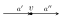
\includegraphics{figures/c12-fig04.svg}
\end{center}

It is trivial to check that the so-defined vector space does not depend on the
choice of cell decomposition (up to a canonical isomorphism); namely,
\begin{equation}\label{e:ZAI-ZAS1}
  \begin{aligned}
    Z_A(I)&=A\otimes_A A\otimes_A \dots \otimes_A A\simeq A\\
    Z_A(S^1)&\simeq A/[A,A].
  \end{aligned}
\end{equation}

If $I$ is an interval, then $Z_A(I)$ is an $A$-bimodule; thus, if we consider
$I$ as a cobordism $\bullet^+\to \bullet^+$, then $Z_A(I)$ is a morphism $A\to
A$ in $\Alg$. We can also consider $I$ as a cobordism
$\bullet^+\sqcup\bullet^-\cob{}\varnothing$, and $Z_A(I)$ as a right module
over $A\otimes A^\op$, or consider $I$ as a cobordism
$\varnothing\cob{}\bullet^+\sqcup\bullet^-$, and $Z_A(I)$ as a left module over
$A\otimes A^\op$.


We can now define $Z_A$ for a 2-cobordism. First, let $M$ be a 2-manifold with
boundary, considered as a cobordism $N\to \varnothing$, where $N=\ov{\del M}$.
Choose a cell decomposition $K$ of $M$; let $E_{\mathrm{bulk}}$ be the set of
oriented edges inside $M$ (thus, every internal unoriented edge of $K_1$
appears twice in $E_{\mathrm{bulk}}$) and $E_{N}$ be the set of oriented edges
on the boundary (each appearing with orientation inherited from $N=\ov{\del
M}$).

Let us modify \eqref{e:fhk-state-sum} and define
\begin{equation}\label{e:fhk-state-sum2}
  Z_A(M,K)= \Bigl(\bigotimes_F \< \, \>_F\Bigr)
  \Bigl(\prod_v(w^{-1}_v) \Bigr)e_M\colon A^{\otimes E_N}\to \kk.
\end{equation}
(note that $e_M\in A^{\otimes E_{\mathrm{bulk}}}$, and $\bigotimes_F \< \, \>_F$ is
a map $A^{\otimes E_{\mathrm{bulk}}\sqcup E_N}\to \kk$). Note that we only take the
product $\prod_v w^{-1}_v$ over \emph{internal} vertices of $K$ and do
not include the vertices on the boundary.

\begin{theorem}\label{t:fhk2}
  \par\noindent
  \begin{enumerate}
    \item The linear map $A^{\otimes E_N}\to \kk$
      defined by \eqref{e:fhk-state-sum2} descends to a
      map $Z_A(N)\to \kk$.
    \item The so-defined operator is independent of the choice of a cell
      decomposition of $M$.
    \item For a closed oriented one-dimensional manifold $N$, let
      $M=N\times I$ considered as a cobordism $N\sqcup \ov{N}\to
       \varnothing$. Then the map
    \begin{equation}\label{e:fhk-pairing}
      Z_A(N\times I)\colon Z_A(N)\otimes Z_A(\ov{N})\to \kk
    \end{equation}
    defined by \eqref{e:fhk-state-sum2}, is a non-degenerate bilinear pairing.
  \end{enumerate}
\end{theorem}
We leave the proof of this theorem to the reader; it is an easy
modification of the proof of \thref{t:fhk1}.

Since the pairing \eqref{e:fhk-pairing} is non-degenerate, it can be used to
identify $Z_A(\ov{N})\simeq (Z_A(N))^*$. In particular, it shows that if $M$ is
a cobordism $N_1\cob{M}N_2$ --- which can also be considered as a cobordism
$N_1\sqcup \ov{N_2}\cob{} \varnothing$ --- then $Z_A(M)\colon Z_A(N_1)\otimes
Z_A(\ov{N_2}) \to \kk$ can also be considered as an operator $Z_A(N_1)\otimes
Z_A(N_2)^*\to\kk$, or equivalently, as an operator $Z_A(N_1)\to Z_A(N_2)$; more
formally, for such a cobordism we define $Z_A(M)\colon Z_A(N_1)\to
Z_A(N_2)$ by
\begin{equation}\label{e:fhk-state-sum3}
  \<Z_A(M)x, y\>= Z_A(M)(x\otimes y), \qquad x \in Z_A(N_1), y \in Z_A(\ov{N_2})
\end{equation}
where $\<\, , \,\>$ is the pairing \eqref{e:fhk-pairing}.

\begin{theorem}\label{t:latticeTQFT}
  Formulas \eqref{e:fhk-state-sum2}, \eqref{e:fhk-state-sum3} define a
  (non-extended) 2-dimensional TQFT.
\end{theorem}

\begin{example}\label{x:lattice-disk}
  Let $D$ be a disk considered as a cobordism $S^1\to\varnothing$. Then
  $Z_A\colon A/[A,A]\to \kk$ is given by the counit of the Frobenius algebra:
  $Z_A(x)=\eps(x)$.
\end{example}
\begin{example}\label{x:lattice-cylinder}
  Let $M=S^1\times I$ be the cylinder considered as a cobordism
  $S^1\sqcup S^1\to \varnothing$. Choosing a decomposition of the cylinder
  obtained by gluing together two sides of the rectangle, we see that in
  this case we have
  $$
    Z_A(M)(a\otimes b)=\sum \eps (ax_ibx^i)
    =\sum \eps(w^{-1} x_jax^jx_i b x^i).
  $$
\end{example}
\begin{exercise}\label{ec:lattice-pants}
  Show that 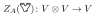
\includegraphics{figures/c12-eqfig02.svg}, where $V=Z_A(S^1)=A/[A,A]$,
  is given by
  $$
    Z_A([a]\otimes[b])=\sum [a x_i b x^i].
  $$
\end{exercise}

Comparing it with \thref{t:centerTQFT}, which gave an explicit description of
the (non-extended) TQFT constructed using Morse decompositions of cobordisms,
we see that these two descriptions match.


Finally, let us define an $Z_A$ as an extended TQFT. We have already defined
$Z$ for 0-dimensional manifolds and 1d cobordisms; thus, to complete the story,
we need to define $Z_A(M)$ for a 2-cobordism, i.e., a 2-manifold with corners
(see \deref{d:2-cobordism}).

\begin{center}
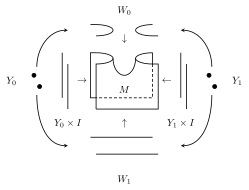
\includegraphics{figures/c12-fig05.svg}
\end{center}


To do that, note that in this case, boundary $\del M$ consists of 3 pieces
(possibly disconnected): $W_0$ (top), $W_1$ (bottom), and ``vertical'' boundary
$Y\times I$, where $Y=Y_0\sqcup Y_1$.

Choosing a cell decomposition $K$ of $M$ such that each corner is a vertex of
that decomposition and using again the formula \eqref{e:fhk-state-sum2}, we can
define
$$
\tilde Z_A(M,K)\colon A^{\otimes E_\ttop}\otimes A^{\otimes E_\bbot}
                \otimes A^{\otimes E_v} \to \kk
$$
where $E_\ttop$, $E_\bbot$, $E_v$ are oriented edges at top, bottom, and
vertical parts of the boundary respectively.

Now, for each vertical edge $e\in E_v$, take vector $1\in A_e$. This
defines a vector $1_v\in A^{\otimes E_v}$. Define
\begin{equation}\label{e:fhk-state-sum3}
  \begin{aligned}
    Z_A(M,K)\colon A^{\otimes E_\ttop}\otimes A^{\otimes E_\bbot}&\to \kk\\
    Z_A(M,K) (a_\ttop\otimes a_\bbot)&=
            \tilde Z_A(a_\ttop\otimes a_\bbot \otimes 1_v).
  \end{aligned}
\end{equation}

% we get the following result.
%\begin{theorem}\label{t:latticeTQFT2}
% For a separable symmetric Frobenius algebra $A$,
% the \textup{(}non-extended\textup{)} TQFT defined by state-sum formulas
% \eqref{e:fhk-state-sum2}, \eqref{e:fhk-state-sum3} coincides with the
% \textup{(}non-extended\textup{)} TQFT defined in \chref{c:2d-extended}.
%\end{theorem}


%%%%%%%%%%%%%%%%%%%%%%%%%%%%%%%%%%%%%%%
\section{Finite group gauge theory as lattice theory}\label{s:lattice-gauge}
Let us consider a special example, which we have already discussed using a
different approach in \exref{x:DW-extended}, namely when the algebra $A=\kk[G]$
is the group algebra of a finite group $G$ and Frobenius structure is given by
$$
  \eps(g)=\de_{g,1} = \frac{1}{|G|}\tr_R(g), \qquad g\in G,
$$
where $R$ is the regular representation.

In this case the element $e=\sum x_i\otimes x^i\in A\otimes A$ is given by
$$
  e=\sum_{g\in G}g\otimes g^{-1}
$$
so that $w=|G|$.

In this case, the map $\<\, , \,\>$ is given by
$$
\<g_1, \dots, g_k\>=\begin{cases}
                     1, & g_1\dots g_k=1\\
                     0, & \text{otherwise}
                   \end{cases}
$$
Thus, one easily sees that for a closed 2-manifold $M$
the state-sum \eqref{e:fhk-state-sum} becomes
$$
Z_A(M,K)=\frac{1}{|G|^V} \sum_{c} 1
$$
where $V$ is the number of vertices of $K$ and  the sum is over all
``colorings'' of edges, i.e., ways of assigning a group element $g_r$ to each
oriented edge $r$ so that for two opposite orientations of the same edge,
$g_{r'}=g_{r''}^{-1}$ and such that the product of colors over the boundary of
any 2-cell is equal to 1.

One easily sees that it is a discrete version of a connection in $G$-bundles:
without the factor $\frac{1}{|G|^V}$, this counts $G$-bundles on $M$ together
with trivializations at every vertex. Thus, dividing by $|G|^V$ exactly gives
the number of $G$-bundles on $M$ counted as in \chref{c:DW}; in other words,
this recovers the Dijkgraaf--Witten TQFT.

